\documentclass[11pt]{article}
\usepackage[a4paper,margin=1in]{geometry}
\usepackage{graphicx}
\usepackage{array}
\usepackage{longtable}
\usepackage{booktabs}
\usepackage{caption}
\captionsetup{labelformat=empty}
\begin{document}
\begin{center}\Large Engineered Feature Formulas\end{center}
\vspace{0.5em}
\setlength{\extrarowheight}{2pt}
\begin{longtable}{@{}p{0.28\linewidth} p{0.68\linewidth}@{}}
\toprule
\textbf{Feature} & \textbf{Formula} \\
\midrule
\endfirsthead
\toprule
\textbf{Feature} & \textbf{Formula} \\
\midrule
\endhead
\bottomrule
\endfoot
Absolute latitude & 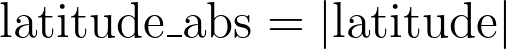
\includegraphics[height=18mm]{figures/formulas/absolute_latitude.png} \\
Air pressure from elevation & 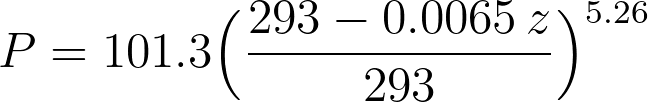
\includegraphics[height=18mm]{figures/formulas/air_pressure_from_elevation.png} \\
Aridity index & 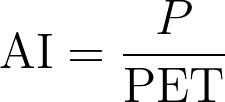
\includegraphics[height=18mm]{figures/formulas/aridity_index.png} \\
Clear sky shortwave & 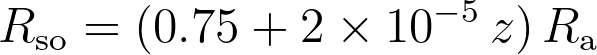
\includegraphics[height=18mm]{figures/formulas/clear_sky_shortwave.png} \\
Clear sky shortwave radiation & 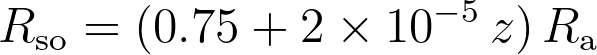
\includegraphics[height=18mm]{figures/formulas/clear_sky_shortwave_radiation.png} \\
Daylight hours & 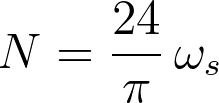
\includegraphics[height=18mm]{figures/formulas/daylight_hours.png} \\
Extraterrestrial radiation & 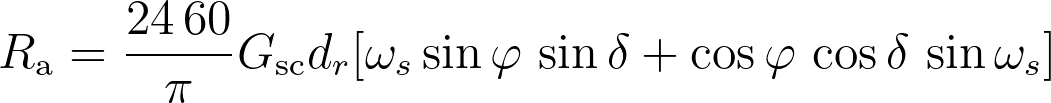
\includegraphics[height=18mm]{figures/formulas/extraterrestrial_radiation.png} \\
Net longwave daily & 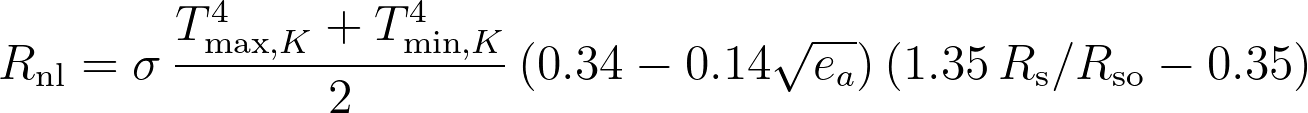
\includegraphics[height=18mm]{figures/formulas/net_longwave_daily.png} \\
Net longwave sub daily & 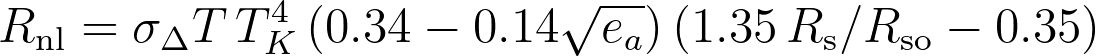
\includegraphics[height=18mm]{figures/formulas/net_longwave_sub_daily.png} \\
Net radiation & 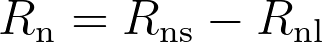
\includegraphics[height=18mm]{figures/formulas/net_radiation.png} \\
Net shortwave & 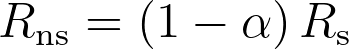
\includegraphics[height=18mm]{figures/formulas/net_shortwave.png} \\
Oudin pet proxy & 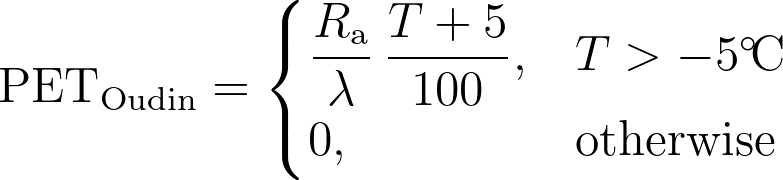
\includegraphics[height=18mm]{figures/formulas/oudin_pet_proxy.png} \\
Ppfd if derived from shortwave & 
\includegraphics[height=18mm]{figures/formulas/ppfd_if_derived_from_shortwave.png} \\
Sapwood to leaf area ratio & 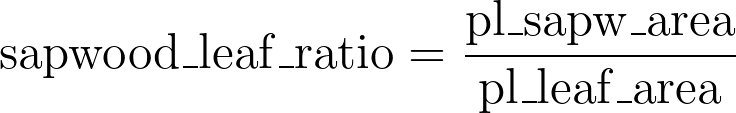
\includegraphics[height=18mm]{figures/formulas/sapwood_to_leaf_area_ratio.png} \\
Tree volume index & 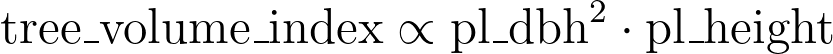
\includegraphics[height=18mm]{figures/formulas/tree_volume_index.png} \\
Vapor pressure deficit & 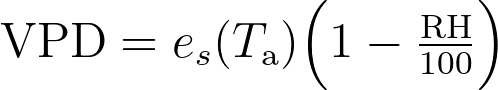
\includegraphics[height=18mm]{figures/formulas/vapor_pressure_deficit.png} \\
\end{longtable}
\end{document}
